\documentclass{beamer}
\usepackage[utf8]{inputenc}

\usetheme{CambridgeUS}
\usecolortheme{beaver}

% --------------------------------------------------------------------- %

\title[MLDM - Project Work]{Machine Learning and Data Mining}
\subtitle{\textbf{Project Work}}

\author{Alessandro Tutone}
\institute[UniBo]{\textit{Alma Mater Studiorum}, Università degli Studi di Bologna}
\date{2025}
\logo{
\includegraphics[height=1.5cm]{imgs/unibo.png}}

% --------------------------------------------------------------------- %

\begin{document}

\frame{\titlepage}

\begin{frame}
\frametitle{Table of Contents}
\tableofcontents
\end{frame}

% --------------------------------------------------------------------- %

\section{Introduction}

\begin{frame}
\frametitle{Task Description}
\textbf{Objective:} Identify which customers \textit{will make a specific transaction in the future}, regardless of the amount of money transacted. 
\newline\\
\textbf{Data structure:} Same structure used for the \textit{real data}
\newline\\
\textbf{Type of classification:} \textit{Binary}
\begin{figure}
\centering
    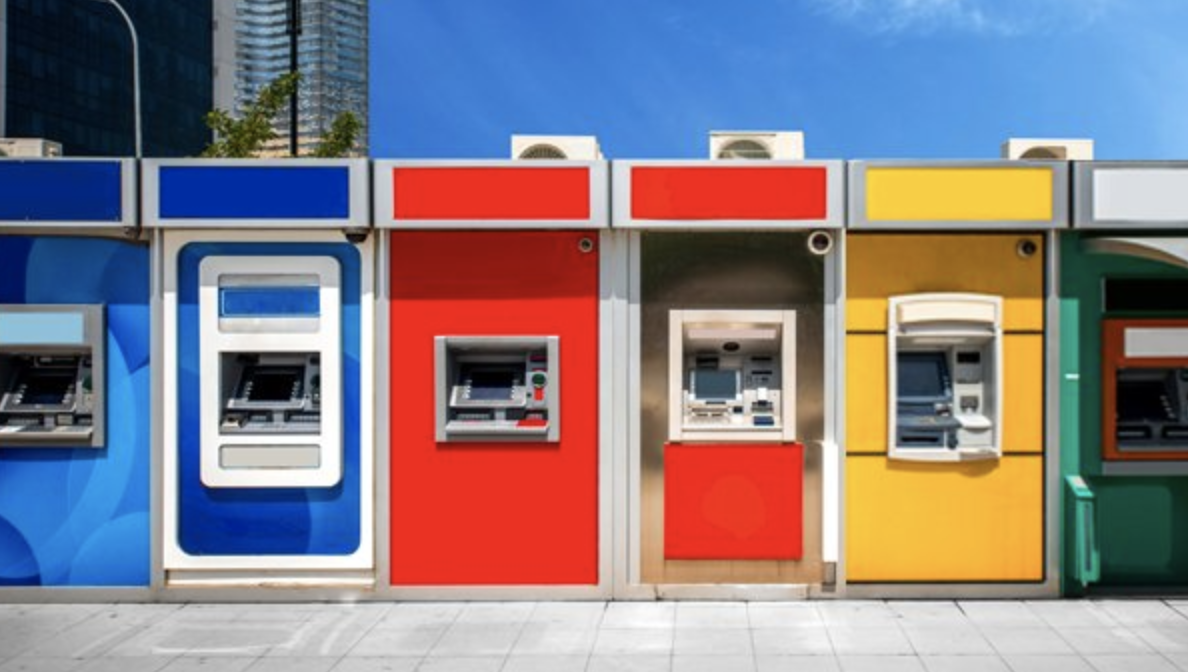
\includegraphics[width=0.6\textwidth]{imgs/task.png}
    \label{fig:task}
\end{figure}
\end{frame}

\begin{frame}
\frametitle{Dataset Description}
\textbf{Anonymized dataset} containing \textit{numeric feature} variables, the \textit{binary target} column, and a \textit{string ID\_code} column.
\newline\\
The task is to predict the value of \textbf{\textit{target column}} in the test set.
\newline\\
\underline{\textbf{File descriptions:}}
\begin{itemize}
    \item \textit{\textbf{train.csv}} - the training set.
    \item \textbf{\textit{test.csv}} - the test set.
    \item \textit{\textbf{sample\_submission.csv}} - a sample submission file.
\end{itemize}
\end{frame}

% -------------------------------------- %

\section{Data exploration}

\begin{frame}
\frametitle{Training dataset}
Lets take a look inside the file \textit{\textbf{train.csv}}
\begin{figure}
\centering
    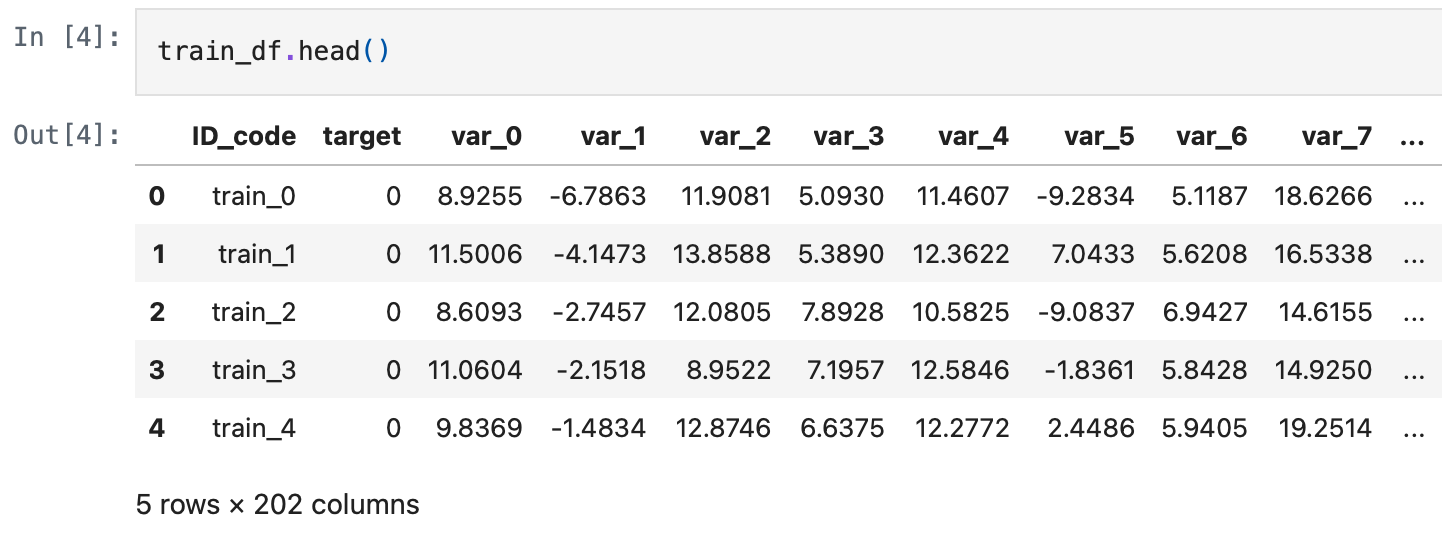
\includegraphics[width=0.9\textwidth]{imgs/training.png}
    \label{fig:training}
\end{figure}
\end{frame}

\begin{frame}
\frametitle{Data distribution}
Considering the \textbf{distributions}, we can learn something new about the data.
\begin{figure}
\centering
    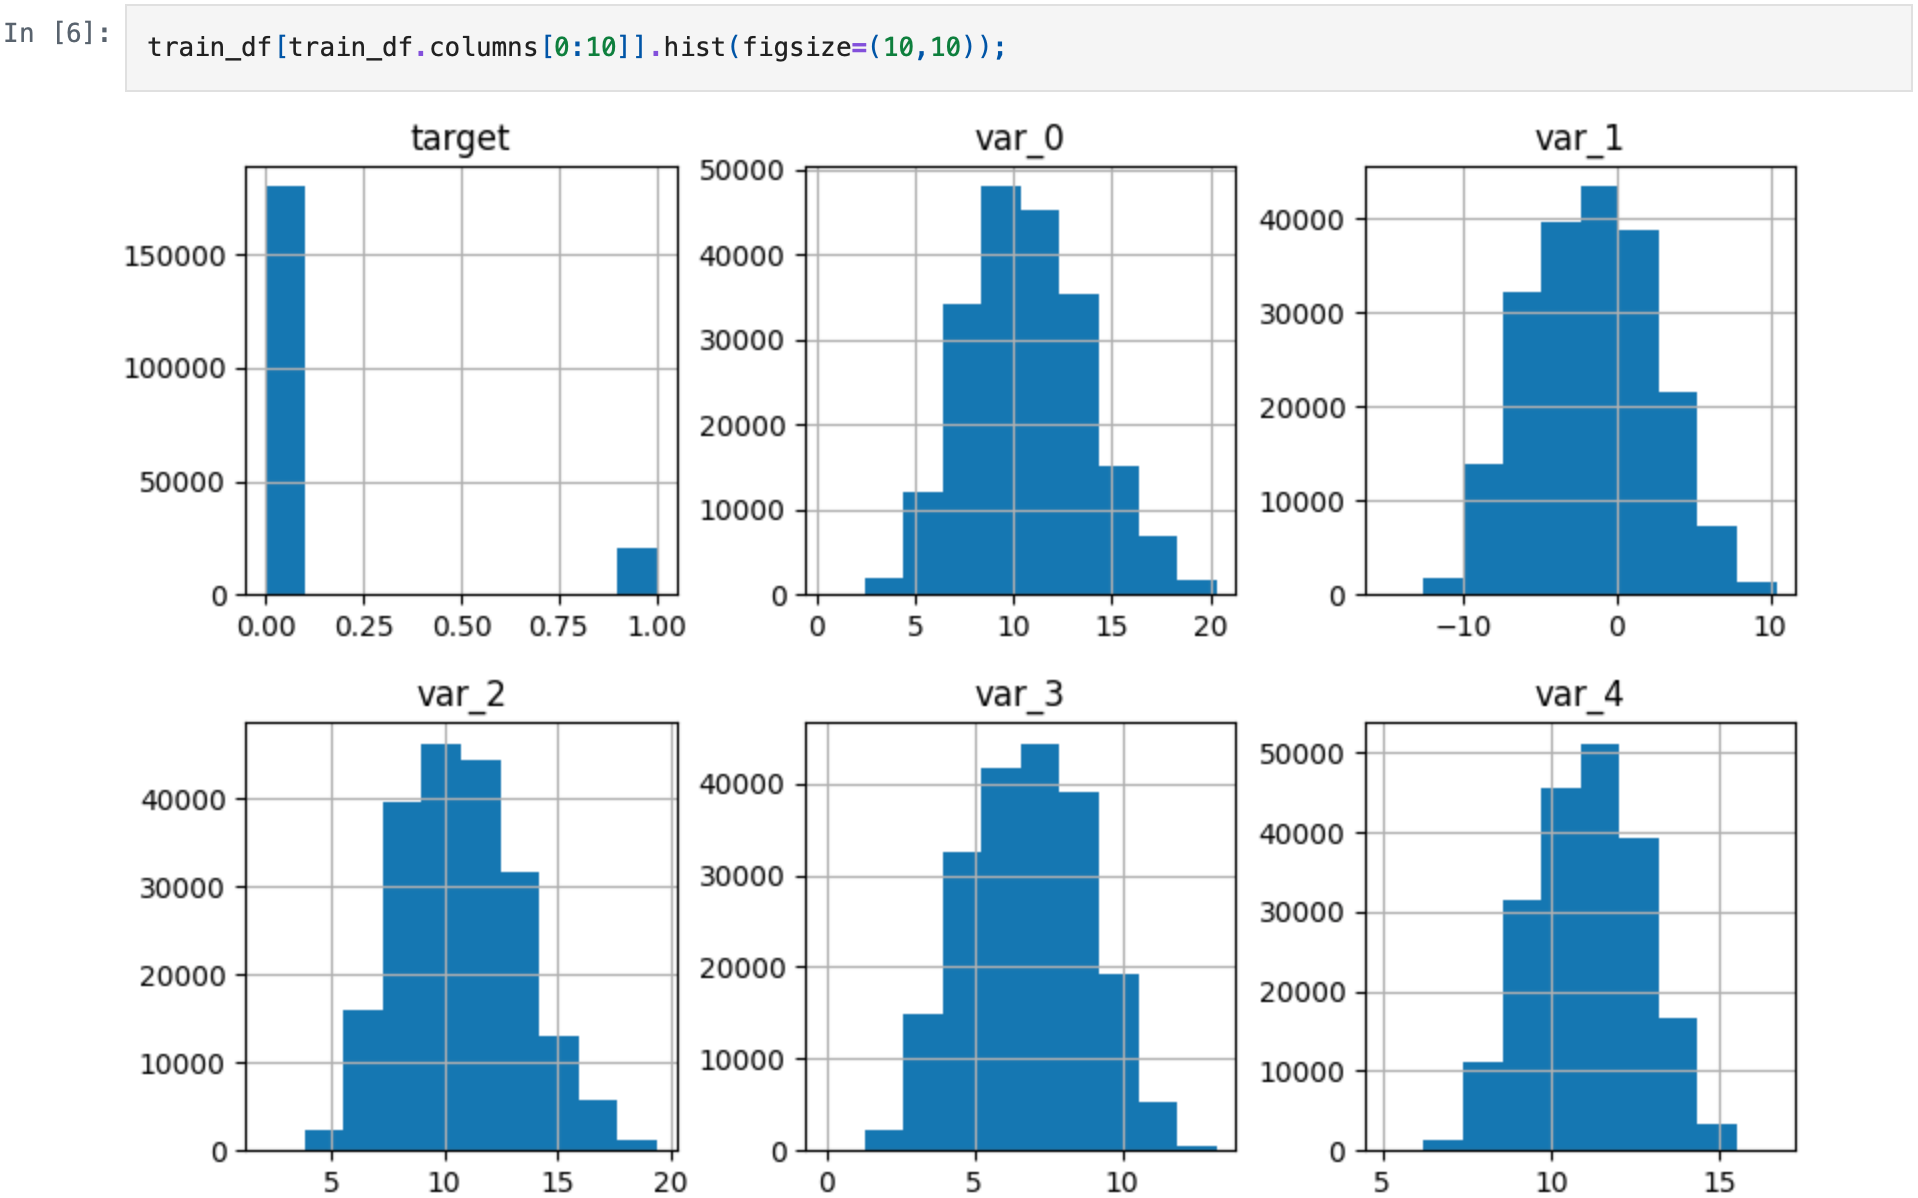
\includegraphics[width=0.79\textwidth]{imgs/distribution.png}
    \label{fig:distribution}
\end{figure}
\end{frame}

\begin{frame}
\frametitle{Data distribution}
All features follow a \textbf{normal distribution}.
\begin{figure}
\centering
    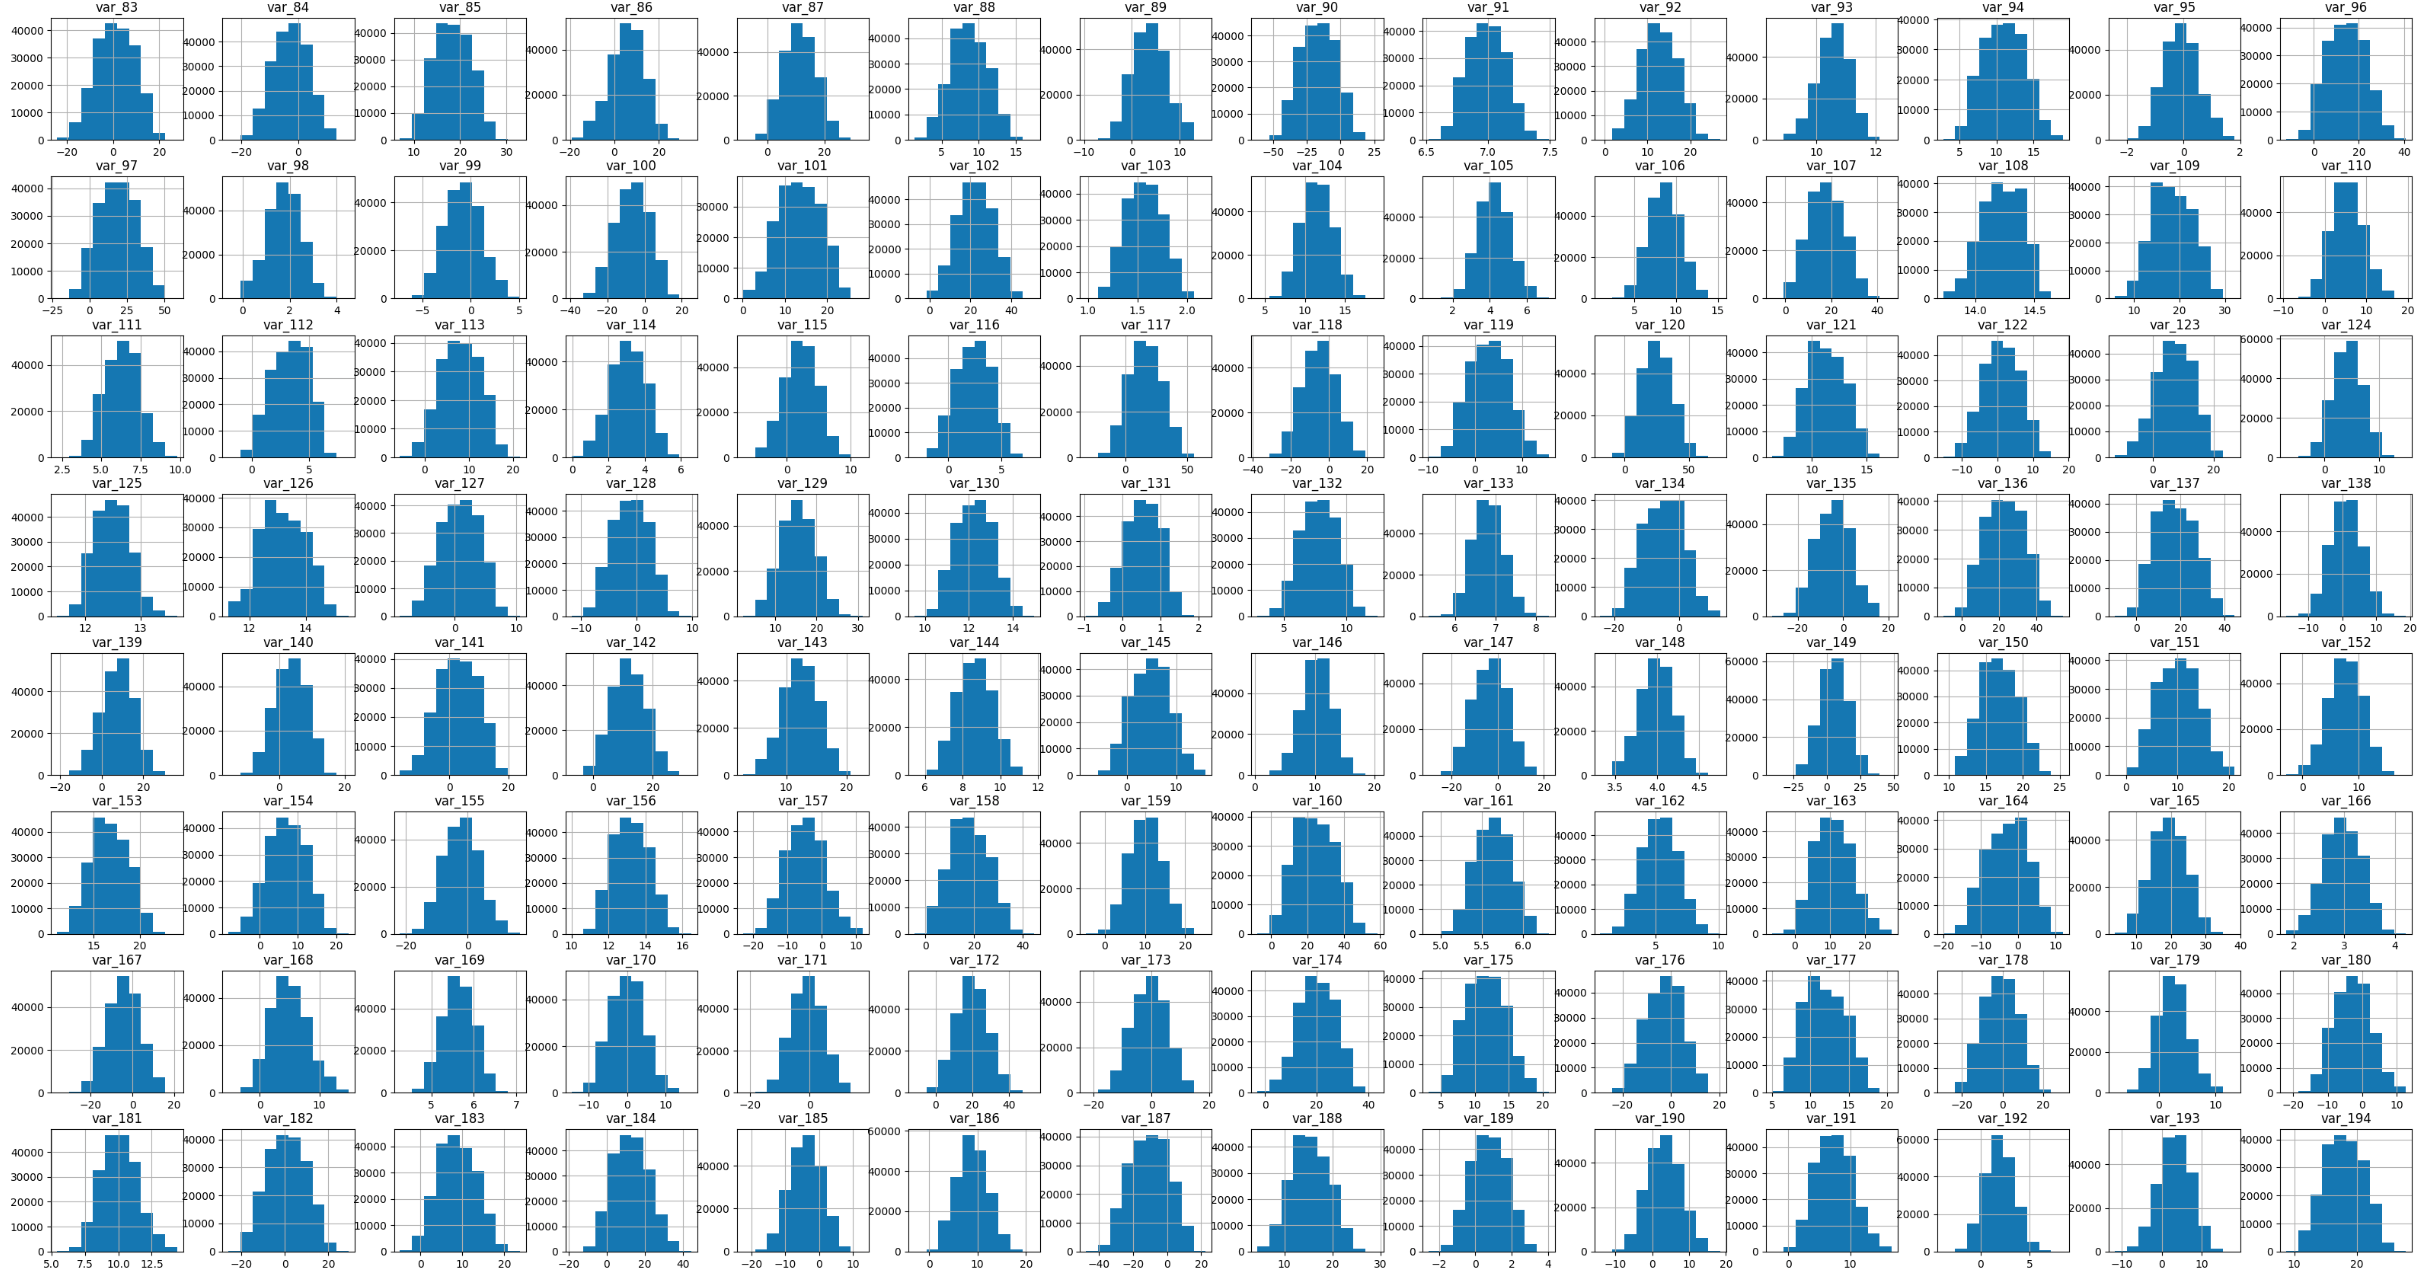
\includegraphics[width=0.79\textwidth]{imgs/distribution_all.png}
    \label{fig:distribution_all}
\end{figure}
\end{frame}

\begin{frame}
\frametitle{Correlation matrix}
What about the \textbf{correlations} between variables?
\begin{figure}
\centering
    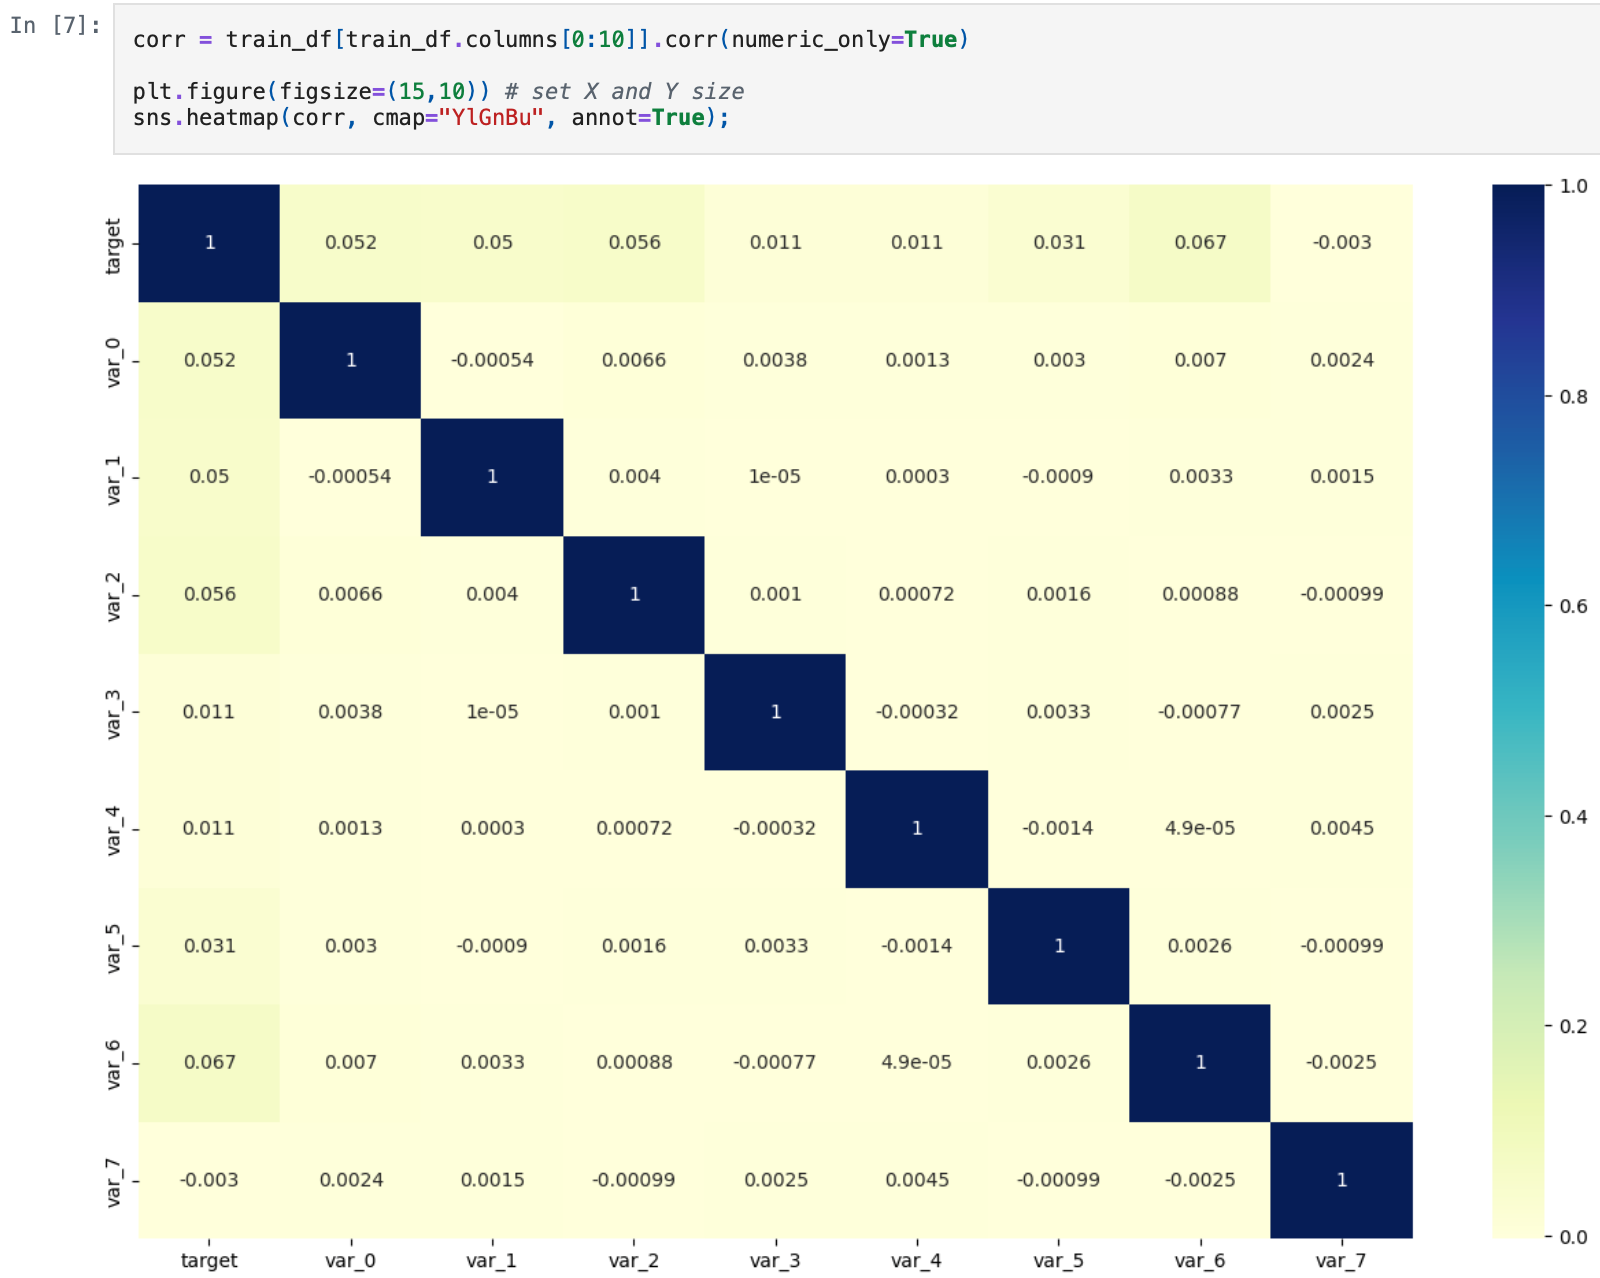
\includegraphics[width=0.7\textwidth]{imgs/matrix.png}
    \label{fig:matrix}
\end{figure}
\end{frame}

% -------------------------------------- %

\section{Training}

\begin{frame}
\frametitle{Train-Test split}
Since the only file that contains the \textbf{\textit{target column}} is \textbf{train.csv}, this dataset is used for both \textit{training} and \textit{testing}
\newline\\
\underline{The data available are divided in the following way:}
\begin{itemize}
    \item 80\% for \textit{\textbf{training}}
    \item 20\% for \textit{\textbf{testing}}
\end{itemize}
\end{frame}

\begin{frame}
\frametitle{First model: \textbf{DecisionTreeClassifier}}
This model works by building a \textbf{tree-like structure} where each node represents a \textit{decision} based on a \textit{feature}. After traversing the \textbf{tree}, the \textbf{\textit{leaf node}} reached represents the \textbf{final prediction} or \textbf{classification}.
\begin{figure}
\centering
    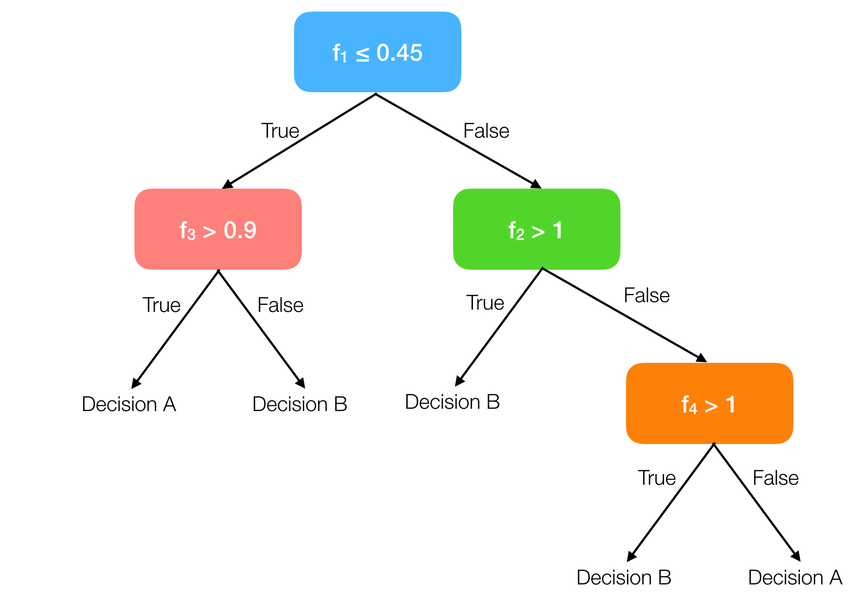
\includegraphics[width=0.65\textwidth]{imgs/dtc.png}
    \label{fig:dtc}
\end{figure}
\end{frame}

\begin{frame}
\frametitle{First model: \textbf{DecisionTreeClassifier}}
A first training, using the \textbf{default parameters}, has been done.
\begin{figure}
\centering
    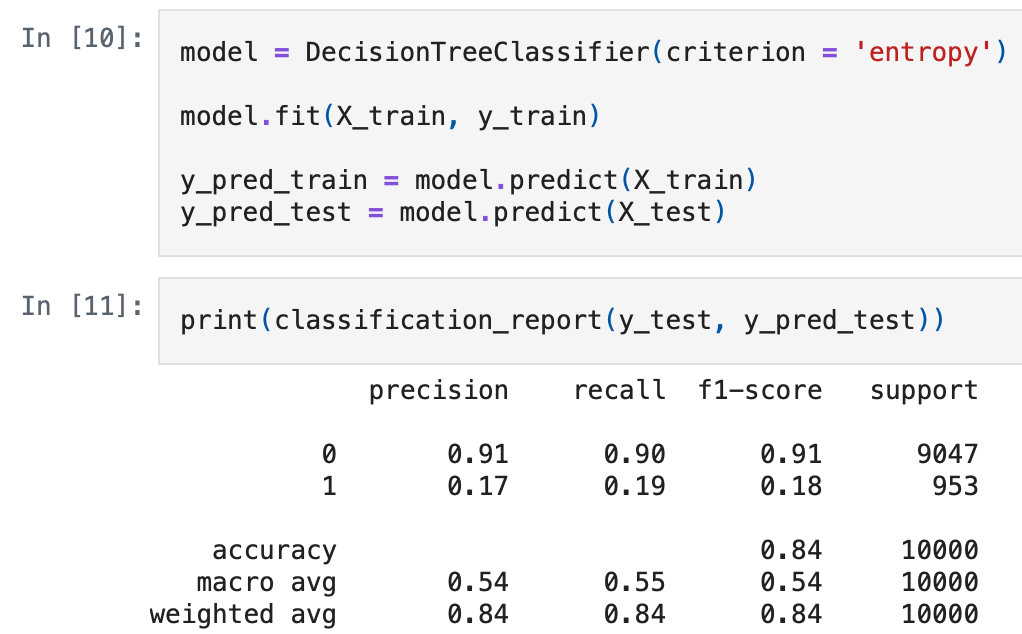
\includegraphics[width=0.68\textwidth]{imgs/dtc_code.png}
    \label{fig:dtc_code}
\end{figure}
\end{frame}

\begin{frame}
\frametitle{Second model: \textbf{GaussianNB}}
This is a classification algorithm that assumes \textit{features} are \textbf{normally distributed} and \textbf{independent}. It calculates the probability of a \textit{feature value} given a \textit{class}, then uses \textbf{Bayes' theorem} to determine the \underline{most likely \textit{class}} for a new data point. 
\begin{figure}
\centering
    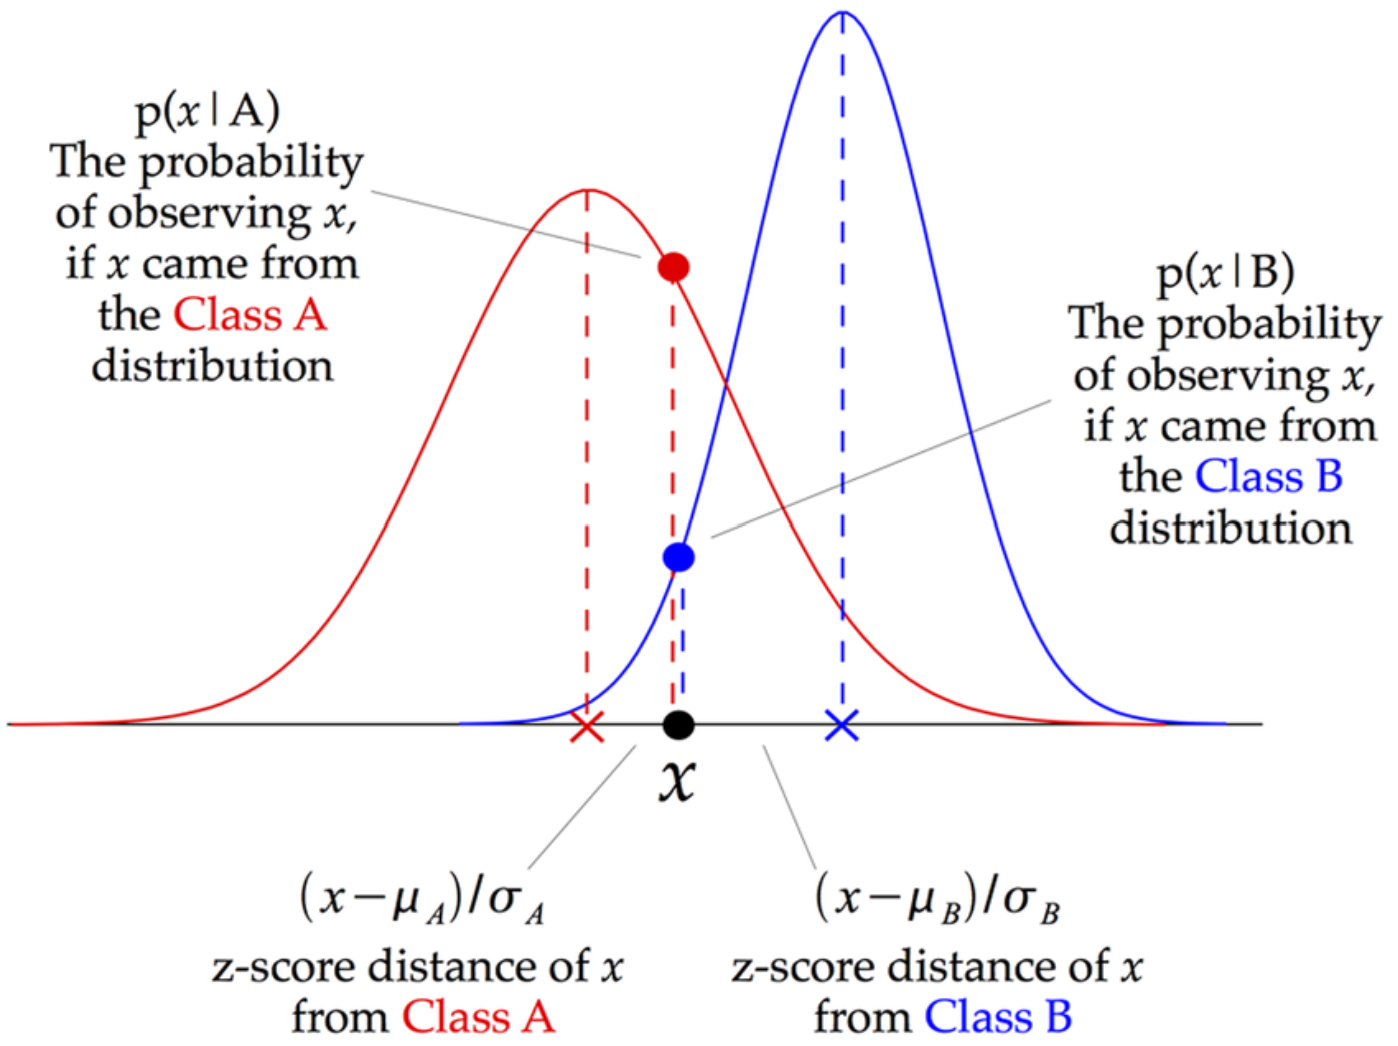
\includegraphics[width=0.55\textwidth]{imgs/gnb.png}
    \label{fig:gnb}
\end{figure}
\end{frame}

\begin{frame}
\frametitle{Second model: \textbf{GaussianNB}}
A first training, using the \textbf{default parameters}, has been done.
\begin{figure}
\centering
    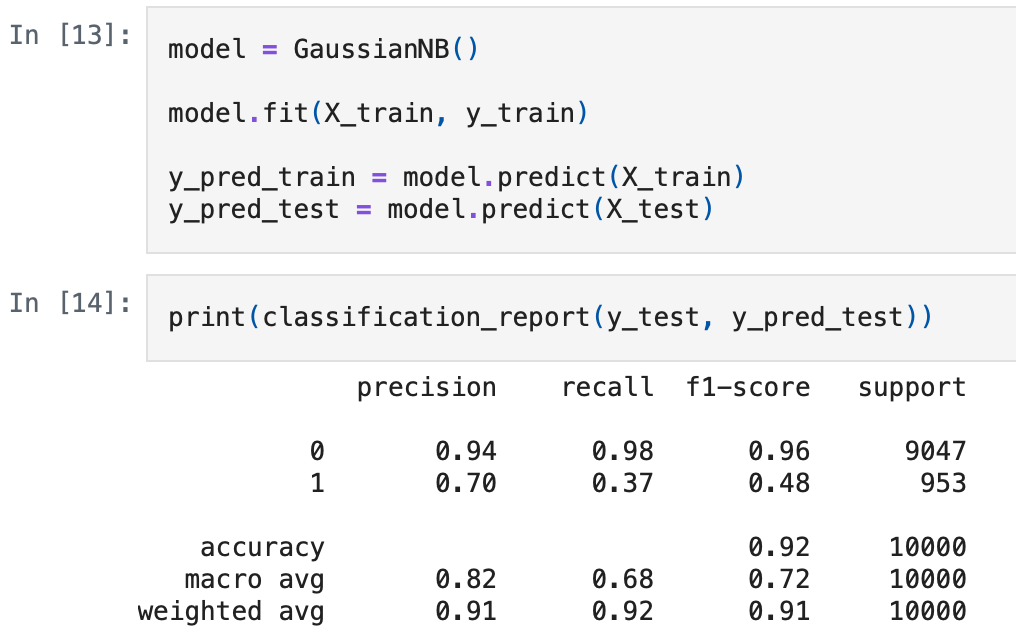
\includegraphics[width=0.7\textwidth]{imgs/gnb_code.png}
    \label{fig:gnb_code}
\end{figure}
\end{frame}

\begin{frame}
\frametitle{Third model: \textbf{KNeighborsClassifier}}
This algorithm is a non-parametric, supervised learning classifier, which uses \textbf{proximity} to make classifications or predictions about the \textit{grouping} of an individual data point.\\
This algorithm assumes that \textit{similar things} exist in \textit{close \textbf{proximity}}
\begin{figure}
\centering
    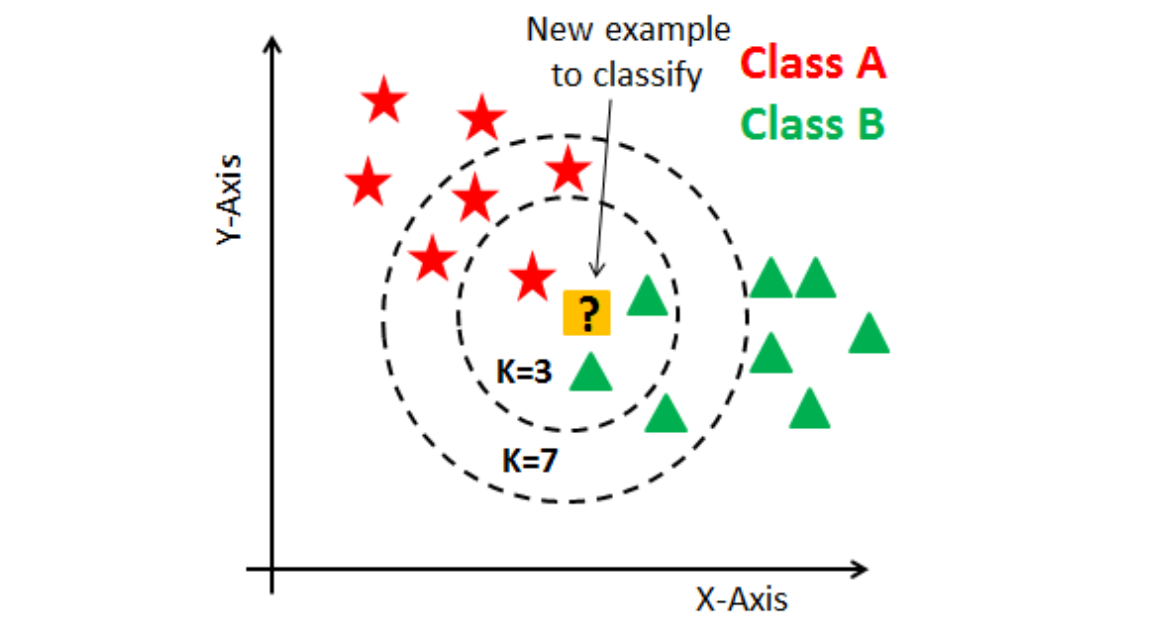
\includegraphics[width=0.7\textwidth]{imgs/knn.png}
    \label{fig:knn}
\end{figure}
\end{frame}

\begin{frame}
\frametitle{Third model: \textbf{KNeighborsClassifier}}
A first training, using the \textbf{default parameters}, has been done.
\begin{figure}
\centering
    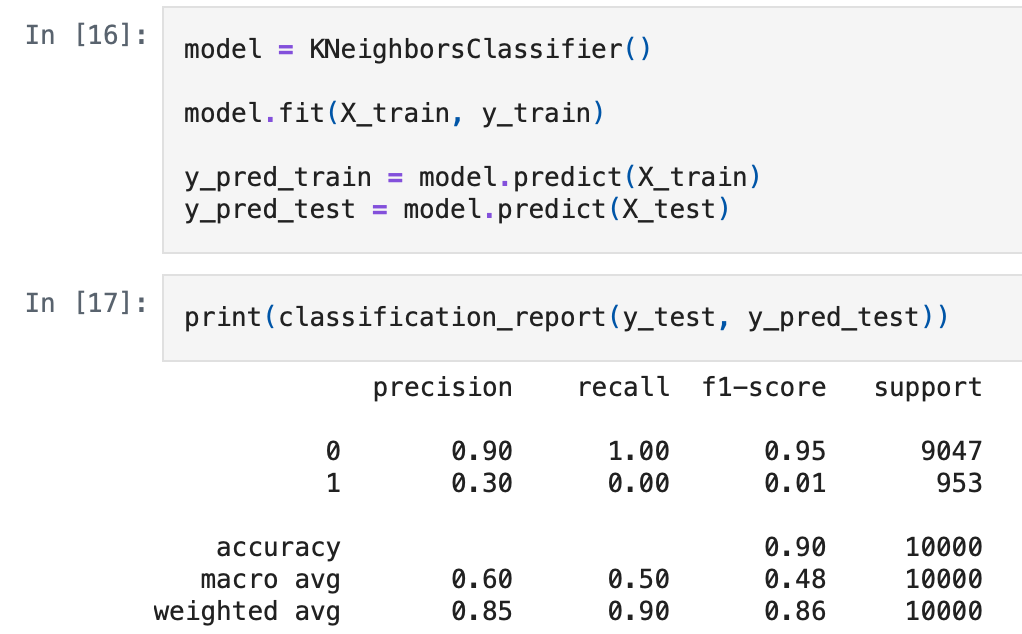
\includegraphics[width=0.7\textwidth]{imgs/knn_code.png}
    \label{fig:knn_code}
\end{figure}
\end{frame}

% -------------------------------------- %

\section{Testing}

\begin{frame}
\frametitle{Comparing all models}
The code used for comparing all the \textbf{models} (with different \textit{parameters}):
\begin{figure}
\centering
    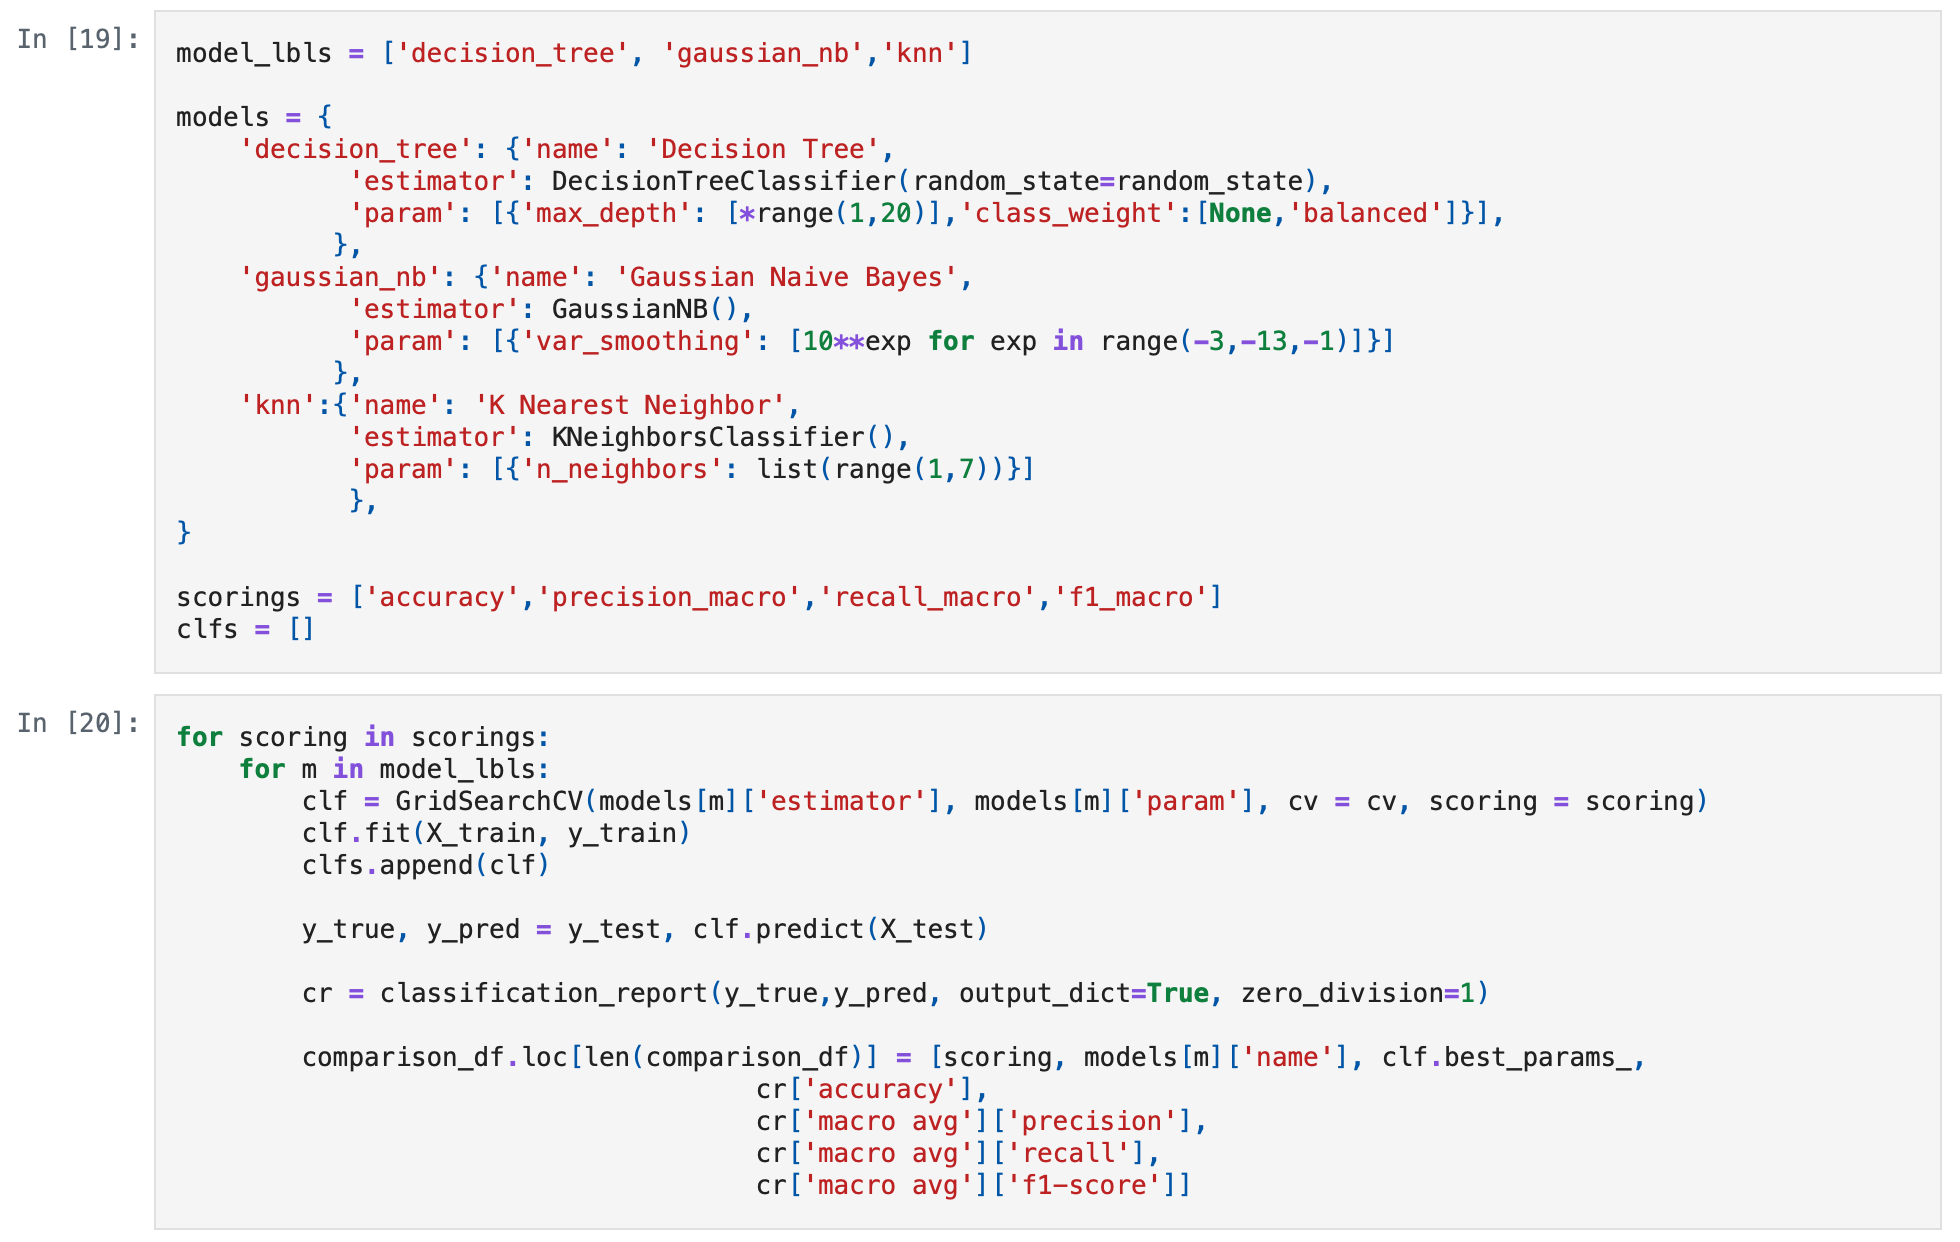
\includegraphics[width=0.78\textwidth]{imgs/comparisons.png}
    \label{fig:comparisons}
\end{figure}
\end{frame}

\begin{frame}
\frametitle{Comparing all models}
Operating a \textbf{grid search} with all \textit{models}, and comparing them using different \textbf{metrics}, it is possible to find \underline{the model that stands out.}
\begin{figure}
\centering
    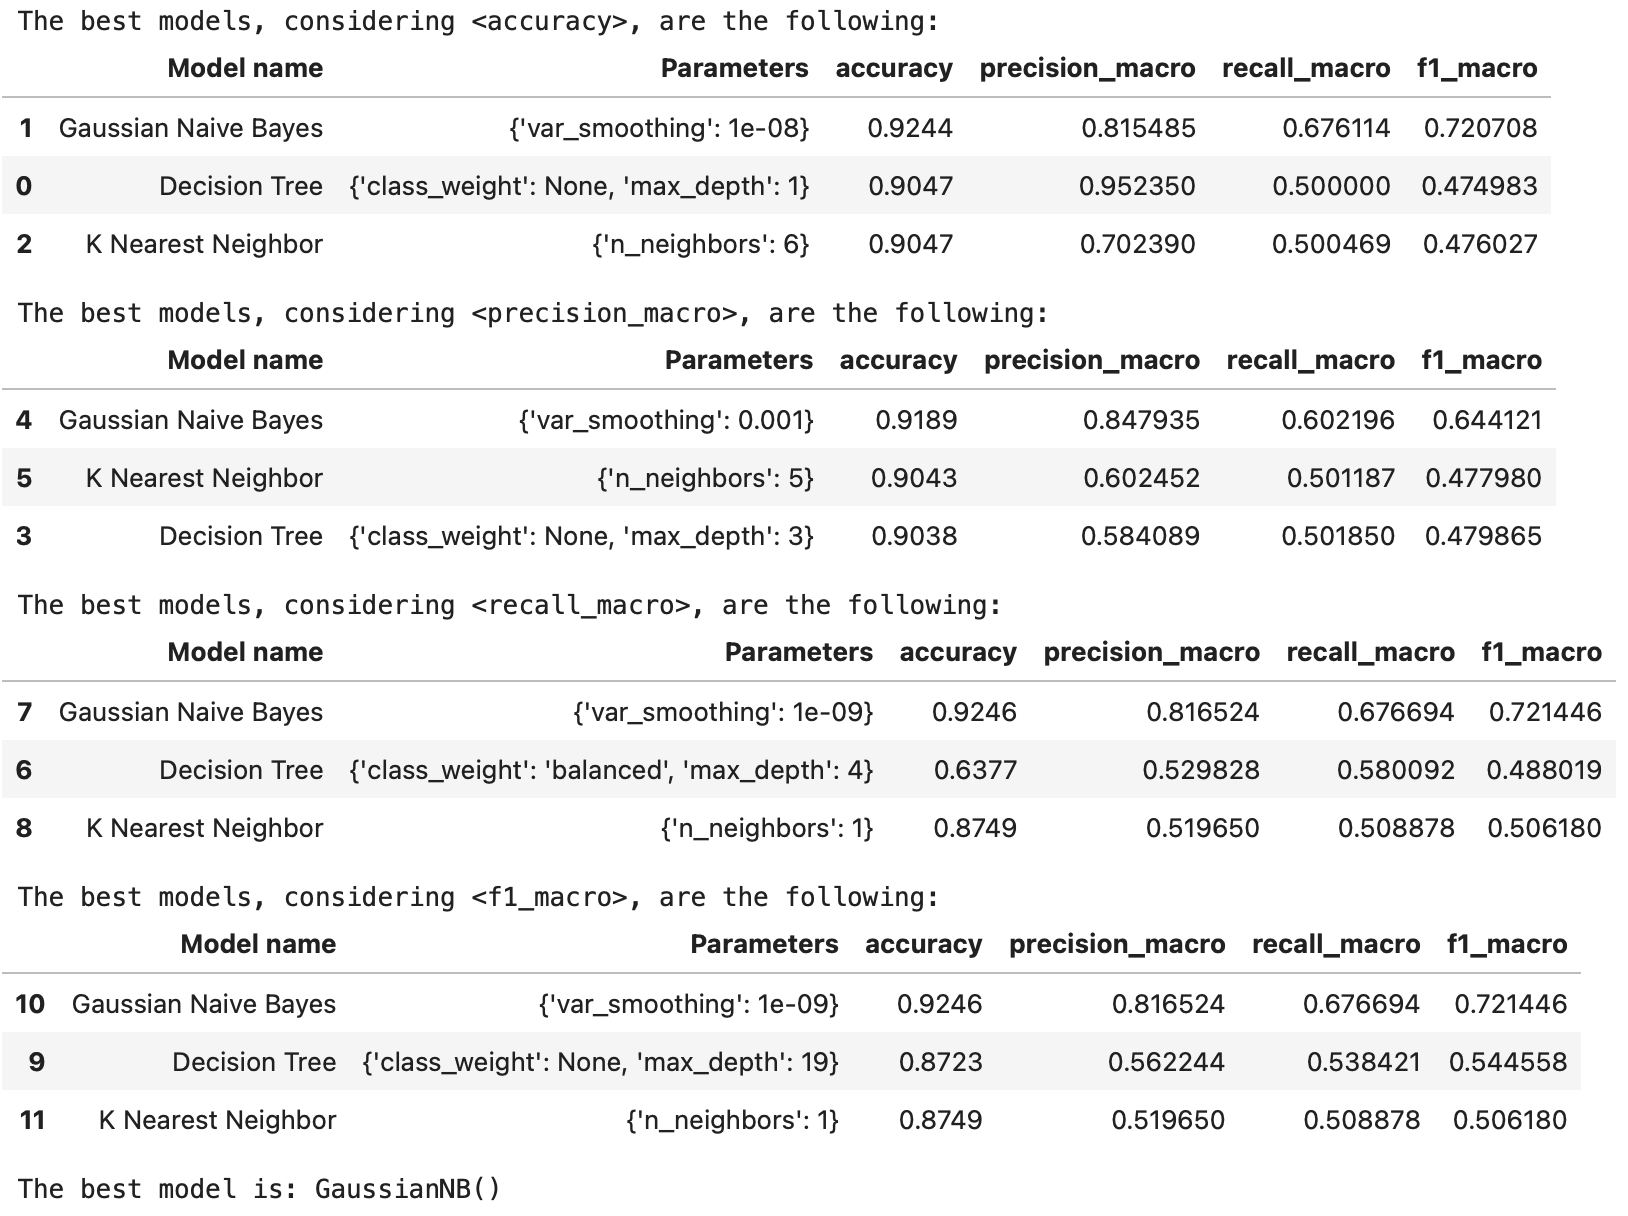
\includegraphics[width=0.7\textwidth]{imgs/testing.png}
    \label{fig:testing}
\end{figure}
\end{frame}

% -------------------------------------- %

\section{Results}

\begin{frame}
\frametitle{The best model}
After all the comparisons, the best model has been found: the metric used to pick the best one is the \textbf{F1-Score}.
\newline\\
\textbf{Best model:} \textit{GaussianNB(var\_smoothing = 1e-09)}
\newline\\
To speed up the computations, all the \textbf{trainings} before have been done with a \underline{smaller number of samples} with respect to the all available samples for \textbf{training}. 
\newline\\
Now it is possible to operate a \underline{\textbf{full training} on the best model}.
\end{frame}

\begin{frame}
\frametitle{Final results}
After a complete training (using all the \textbf{160.000} samples) the results obtained with the \textbf{best model} are the following:
\begin{figure}
\centering
    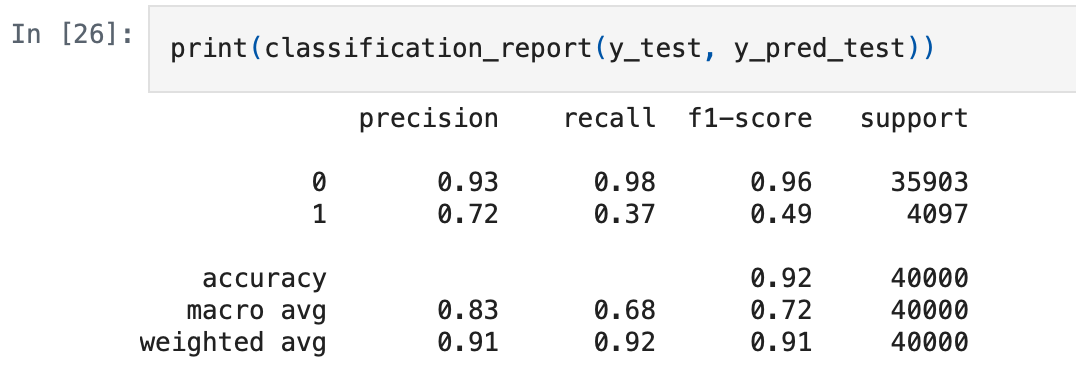
\includegraphics[width=0.89\textwidth]{imgs/results.png}
    \label{fig:results}
\end{figure}
\end{frame}

\end{document}